\textbf{Цель работы:}  исследование резонанса напряжений в последовательном колебательном контуре с изменяемой ёмкостью, получение ампилтудно-частотных и фазово-частотных характеристик, определение основных параметров контура. 
\\\indent\textbf{Оборудование:} генератор сигналов, источник напряжения, нагрузкой которого является последовательный колебательный контур с переменной ёмкостью, двухканальный осциллограф, цифровые вольмтетры. 
 

\section*{Экспериментальная установка}

\begin{figure}[h!]
    \centering
    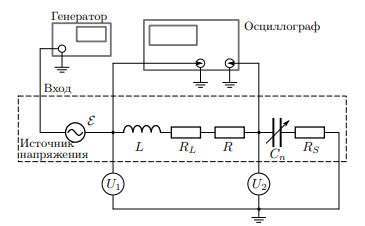
\includegraphics[width=12cm]{setup.png}
    \caption{Схема установки}
\end{figure}

Источник напряжения, колебательный контур и блок питания находятся в отдельном корпусе, на котором так же имеется магазин ёмкостей $C_n$.
\begin{table}
        \centering
        \begin{tabular}{|c|c|c|c|c|c|c|c|}
            \hline
            n & $1 $& $2 $& $3 $& $4 $& $5 $& $6 $& $7$ \\\hline 
            $C_n$, нФ & $25.0$ & $33.2$ & $47.5$ & $57.2$ & $67.4$ & $82.1$ & $99.6$ \\\hline
            \multicolumn{8}{|c|}{ $R = 3.45$Ом}\\\hline
        \end{tabular}
        \caption{Велечины ёмкостей $C_n$}
\end{table}


\section*{Теоретические сведения}
\indent Уравнение последовательного колебательного контура с подключенным внешним ЭДС выглядит следующим образом:
\begin{equation}
    \ddot{U_c} + 2\gamma\dot{U_c} + {\omega_0}^2 U_c = {\omega_0}^2\varepsilon_0\cos(\omega t + \varphi)
\end{equation}
Решение такой системы ищется в виде $\overline{U_C}(t) = \overline{U_{C0}}e^{i\omega t}$.
И с учетом того, что импеданс системы можно записать как $Z = Z_0 e^{i\psi}$, где $Z_0 = \sqrt{R^2 + {\left (\omega L - \frac{1}{\omega C}\right )}^2}$\\
Отсюда получаем:
\begin{align}
    I(t)   &= \frac{\varepsilon_0}{Z_0}\cos(\omega t + \phi_0 - \psi);\\
    U_C(t) &= \frac{\varepsilon_0}{Z_0 C\omega}\cos(\omega t + \phi_0 - \psi_C), \psi_C = \psi + \frac{\pi}{2};\\
    U_L(t) &= \frac{\varepsilon_0 L \omega}{Z_0}\cos(\omega t + \phi_0 - \psi_L), \psi_L = \psi - \frac{\pi}{2}
\end{align}
Тогда найдем частоту и соответсвующее ей напряжене при резонансе напряжения на конденсаторе:
\begin{align}
    U_{C\omega}^{\text{рез}} = U_{L\omega}^{\text{рез}} &= \frac{\rho}{R_\sum}\varepsilon_0 {\left ( 1 - \frac{{\rho}^2}{4 R^2}\right)}^{-1/2};\\
    \omega_C^{\text{рез}}  &= \omega_0 {\left ( 1 - \frac{{\rho}^2}{2 R^2}\right )}^{1/2};\\
    \omega_L^{\text{рез}}  &= \omega_0 {\left ( 1 - \frac{{\rho}^2}{2 R^2}\right )}^{-1/2}
\end{align}
Такая колебательная система характеризуется добротностю $Q$.
\begin{equation}
    Q = \frac{1}{2}\sqrt{\frac{\omega_0^2}{\gamma^2} - 1} = \sqrt{\frac{\rho^2}{R_{\sum}^2} - \frac{1}{4}}
\end{equation}
где $\rho = \sqrt{\frac{L}{C}}$ - волновое сопротивление контура, $R_{\sum} = R + R_L + R_S$ - активное сопротивление системы.
При слабом затухании $Q \gg 1 \Rightarrow \gamma \ll \omega_0 \Rightarrow Q \approx \frac{\omega_0}{2\gamma} = \frac{1}{R_{\sum}}\sqrt{\frac{L}{C}} = \frac{\rho}{R_{\sum}} = \frac{1}{\omega_0 C R_{\sum}}$
Выражения для импедансов ёмкости, индуктивности и последовательного контура:
\begin{align}
    Z_C = R_S - \frac{i}{\omega C},\quad
    Z_L = R_L + i\omega L,\quad
    Z   = R_{\sum} + i\left (\omega L - \frac{1}{\omega L}\right )
\end{align}



\section*{Экспериментальные данные}

\indent При резонансе $\omega_0 = \omega$, тогда индуктивность можно вычислить по формуле $L = \frac{1}{4 \pi^2 \nu^2 C}$, добротность колебательного контура определяется по формуле $Q = \frac{U_c^{\text{рез}}}{\varepsilon_0}$, $\rho = \sqrt{\frac{L}{C}}$. Будем придерживаться того, что $Q >> 1$(хотя судя на самом деле не совсем так) и считать суммарное сопротивление как $R_{\sum} = \frac{\rho}{Q}$.
$R_{\text{Smax}} = 10^{-3}\rho$, $R_L = R_{\sum} - R_{\text{Smax}} - R$, $I = \frac{\varepsilon_0}{R{\sum}}$
\begin{table}[h!]
    \centering
    \begin{tabular}{|c|c|c|c|c|c|c|c|c|c|c|}
        \hline
        $C_n$, нФ & $f_{0n}$, кГц & $U_c$, В & $\varepsilon$, В & $L$, мкГн & $Q$ & $\rho$, Ом & $R_{\sum}$, Ом & $R_{\text{Smax}}$, Ом & $R_L$, Ом & $I$, мА\\\hline
        25.0 & 31.3 & 4.93 & 0.2 & 1034.2& 24.6 & 203.40 & 8.25  & 0.20 & 4.60 & 24.24 \\\hline          
        33.2 & 27.1 & 3.27 & 0.2 & 1024.7& 16.4 & 175.60 & 10.74 & 0.18 & 7.11 & 18.62 \\\hline
        47.5 & 23   & 3.86 & 0.2 & 1008.1& 19.3 & 145.67 & 7.55  & 0.15 & 3.95 & 26.50 \\\hline
        57.2 & 21   & 3.40 & 0.2 & 1004.2& 17.0 & 132.50 & 7.80  & 0.13 & 4.21 & 25.66 \\\hline      
        67.4 & 19.4 & 2.78 & 0.2 &  998.6& 13.9 & 121.71 & 8.76  & 0.12 & 5.19 & 22.84 \\\hline
        82.1 & 17.5 & 3.06 & 0.2 & 1007.4& 15.3 & 110.77 & 7.24  & 0.11 & 3.68 & 27.62 \\\hline
        99.6 & 15.9 & 2.83 & 0.2 & 1006.0& 14.2 & 100.50 & 7.10  & 0.10 & 3.55 & 28.16 \\\hline
        \multicolumn{4}{|c|}{Среднее значение}  & 1011.7 & - & - & - & - & 4.61 & -       \\\hline
        \multicolumn{4}{|c|}{Случ. погрешность} &  11.6   & - & - & - & - & 1.14 & -      \\\hline
    \end{tabular}
    \caption{Результаты измерений резонансной частоты и напряжения для разных значений ёмкости при $\varepsilon_0 = 0.2$В}
\end{table}

\begin{table}[h!]
    \centering
    \begin{tabular}{|c|c|c|c|c|c|c|c|c|c|c|}
        \hline
        $C_n$, нФ & $f_{0n}$, кГц & $U_c$, В & $\varepsilon$, В & $L$, мкГн & $Q$ & $\rho$, Ом & $R_{\sum}$, Ом & $R_{\text{Smax}}$, Ом & $R_L$, Ом & $I$, мА\\\hline
        25.0 & 31.18 & 9.47 & 0.4 & 1042.2& 24 & 204.18 & 8.64  & 0.20 & 4.97 & 46.38 \\\hline          
        33.2 & 27.21 & 7.56 & 0.4 & 1030.5& 19 & 176.18 & 9.21  & 0.18 & 5.58 & 43.42 \\\hline
        47.5 & 22.92 & 7.22 & 0.4 & 1015.1& 18 & 146.19 & 8.10  & 0.15 & 4.50 & 49.39 \\\hline
        57.2 & 20.92 & 6.48 & 0.4 & 1011.9& 16 & 133.00 & 8.21  & 0.13 & 4.63 & 48.72 \\\hline      
        67.4 & 19.26 & 5.86 & 0.4 & 1013.1& 15 & 122.60 & 8.37  & 0.12 & 4.80 & 47.80 \\\hline
        82.1 & 17.49 & 5.60 & 0.4 & 1008.6& 14 & 110.84 & 7.92  & 0.11 & 4.36 & 50.52 \\\hline
        99.6 & 15.92 & 5.51 & 0.4 & 1003.4& 14 & 100.37 & 7.29  & 0.10 & 3.73 & 54.90 \\\hline
        \multicolumn{4}{|c|}{Среднее значение}  & 1017.8 & - & - & - & - & 4.65 & -       \\\hline
        \multicolumn{4}{|c|}{Случ. погрешность} & 12.6   & - & - & - & - & 0.52 & -      \\\hline
    \end{tabular}
    \caption{Результаты измерений резонансной частоты и напряжения для разных значений ёмкости при $\varepsilon_0 = 0.4$В}
\end{table}

\indent Сравнивая таблицы, можно сказать, что все характеристики за исключением силы тока в среднем совпадают. Значения же для силы тока различаются примерно в 2 раза, что не удивительно, т.к напряжение тоже было поднято в 2 раза, а остальные значения сохранились.
\\\indent Далее определим амплитудно-частотные характеристики системы для ёмкостей $C_1$ и $C_7$. Данные представлены в таблицах 4,6. По ним так же вычислим добротность и сравинм результаты с прошлыми полученными значениями.
\newpage
\begin{table}[h!]
    \begin{minipage}{0.3\linewidth}
        \begin{tabular}{|c|c|}
            \hline
            $\nu$, кГц  & $U_C$\\\hline
            30560 &  3.00 \\\hline
            30660 &  3.28 \\\hline
            30760 &  3.58 \\\hline
            30860 &  3.93 \\\hline
            30960 &  4.27 \\\hline
            31060 &  4.58 \\\hline
            32160 &  4.81 \\\hline
            31160 &  4.93 \\\hline
            31260 &  4.93 \\\hline
            31360 &  4.81 \\\hline
            31460 &  4.61 \\\hline
            31560 &  4.39 \\\hline
            31660 &  4.12 \\\hline
            31760 &  3.87 \\\hline
            31860 &  3.62 \\\hline
            31960 &  3.38 \\\hline
            32060 &  3.15 \\\hline
            32260 &  2.95 \\\hline
            32360 &  2.76 \\\hline
            32460 &  2.58 \\\hline
        \end{tabular}
        \caption{АЧХ при $C_1$}
    \end{minipage}
    \begin{minipage}{0.7\textwidth}
        \centering
        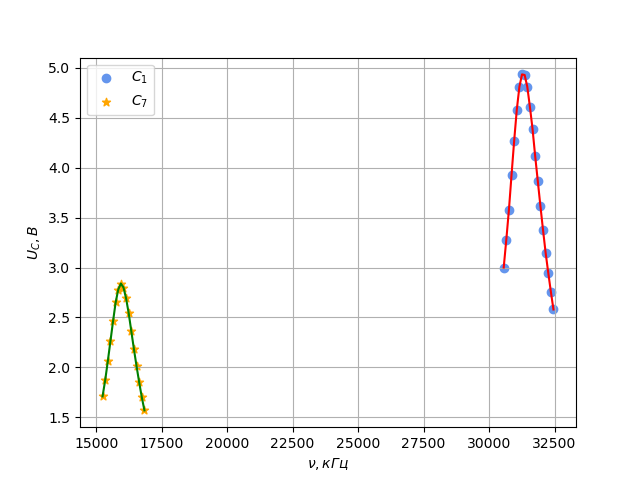
\includegraphics[width=13cm]{./images/plot1.png}
        \caption*{График АЧХ для $C_1$ и $C_7$}
    \end{minipage}
    \begin{minipage}{0.3\linewidth}
        \begin{tabular}{|c|c|}
            \hline
            $\nu$, кГц  & $U_C$\\\hline
            15240 & 1.71 \\\hline
            15340 & 1.87 \\\hline
            15440 & 2.06 \\\hline
            15540 & 2.26 \\\hline
            15640 & 2.46 \\\hline
            15740 & 2.65 \\\hline
            15840 & 2.78 \\\hline
            15940 & 2.84 \\\hline
            16040 & 2.80 \\\hline
            16140 & 2.69 \\\hline
            16240 & 2.54 \\\hline
            16340 & 2.36 \\\hline
            16440 & 2.18 \\\hline
            16540 & 2.01 \\\hline
            16640 & 1.85 \\\hline
            16740 & 1.70 \\\hline
            16840 & 1.57 \\\hline
        \end{tabular}
        \caption{AЧХ при $C_7$}
    \end{minipage}
    \begin{minipage}{0.7\textwidth}
        \centering
        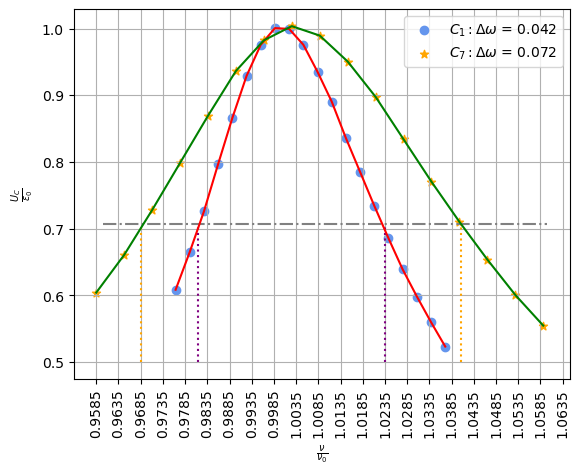
\includegraphics[width=13cm]{./images/plot2.png}
        \caption*{График АЧХ для $C_1$ и $C_7$ в безразмерных координатах}
    \end{minipage}
\end{table}

\begin{table}[h!]
    \begin{minipage}{0.3\linewidth}
        \begin{tabular}{|c|c|c|}
            \hline
            $\nu_{C1}$, кГц & $\nu_{C7}$, кГц  & $x$\\\hline
            29750 & 14150 & 2   \\\hline
            30450 & 14550 & 3   \\\hline
            30700 & 14850 & 4   \\\hline
            30890 & 15150 & 5   \\\hline
            31030 & 15350 & 6   \\\hline
            31160 & 15550 & 7   \\\hline
            31290 & 15610 & 8   \\\hline
            31410 & 15680 & 9   \\\hline
            31580 & 15740 & 10  \\\hline
            31750 & 15840 & 11  \\\hline
            32020 & 15870 & 12  \\\hline
            32440 & 15920 & 13  \\\hline
        \end{tabular}
        \caption{АЧХ при $C_1$}
    \end{minipage}
    \begin{minipage}{0.7\textwidth}
        \centering
        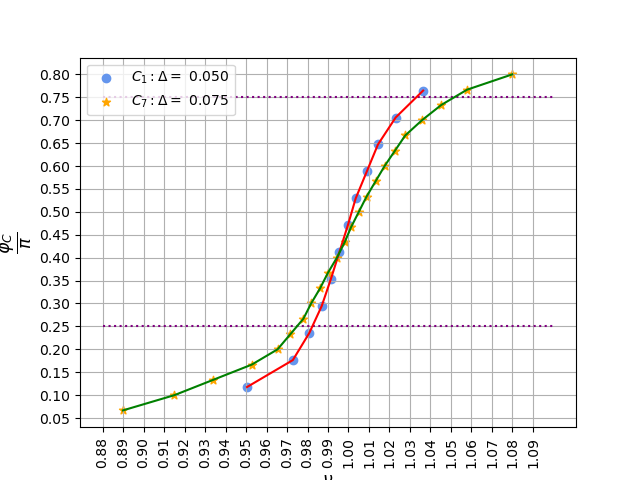
\includegraphics[width=13cm]{./images/plot3.png}
        \caption*{График ФЧХ для $C_1$ и $C_7$}
    \end{minipage}
\end{table} 

\begin{wrapfigure}{r}{0.4\linewidth}
        \centering
        \begin{tabular}{|c|c|c|}
            \hline
            $C_n$ & $C_1$ & $C_7$ \\\hline
            $Q = \frac{U_C^{ \text{рез}}}{\varepsilon_0}$ & 24.6 & 14.2 \\\hline
            $Q = \frac{\omega_0}{\delta \omega}$& 23.81 & 13.88 \\\hline
            $Q = \frac{1}{\Delta \frac{\nu}{\nu_0}}$& 20 & 13.3 \\\hline
        \end{tabular}
        \caption{Сравнение добротностей, посчитанных разными способами}
\end{wrapfigure}
Значение добротности по ФЧХ найдем по ширине кривой, ограниченной занчениями $\frac{\Delta \varphi}{\pi}$ между 0.25 и 0.75.

Теперь рассмотрим график зависимости $R_L(\nu_0)$ (представлен ниже). Видно, что значения $R_L$ откланяются от среднего достаточно сильно ($\approx 25\%$). Причиной такого повидения могут быть скин-эффект (ток течет по меньшему сечению). 
\\
\begin{wrapfigure}{l}{0.9\linewidth}
    \centering
    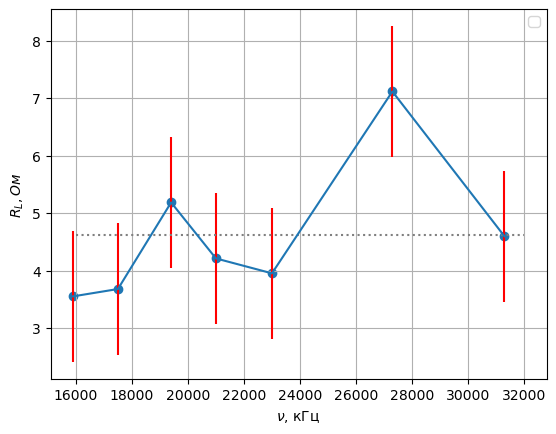
\includegraphics[width=9cm]{./images/plot4.png}
    % \caption*{График $R_L(\nu_0)$}
\end{wrapfigure}

\\\\Оценим погрешности.В случае AЧХ $\sigma_{\frac{\Delta \omega}{\omega}} = 0.005$, тогда $\sigma_Q = \frac{\sigma_{\frac{\Delta \omega}{\omega}}}{{\Delta \omega}^2}$, $\sigma_{Q1} = 2.82$, $\sigma_{Q7} = 0.96$.
Аналогично считается в случае ФЧХ: $\sigma_{Q1} = 4, \sigma_{Q7} = 1.8$.
Видно, что значения для добротности полученные всеми способоми близки и с учетом погрешности совпадают. 
Однако считать $Q$ через ФЧХ менее точно, чем АЧХ.






